\section{Đánh giá ưu, nhược điểm của hệ thống}
    \subsection{Ưu điểm}
        Dựa trên những thành tựu đã nêu, chúng ta có thể kết luận rằng dự án đã đạt được những ưu điểm đáng kể.
        
        \begin{itemize}
            \item \textit{Định nghĩa bài toán và lựa chọn phương pháp giải:} Việc định rõ bài toán và lựa chọn phương pháp giải đặt nền móng cho sự thành công của dự án. Bằng cách này, chúng ta đã có một hướng đi rõ ràng và có thể tiến hành thực hiện mở rộng một cách hiệu quả trong tương lai.
            \item \textit{Xây dựng hệ thống và các chức năng:} Việc xây dựng được hệ thống website BKareer với các chức năng cơ bản cần thiết là một bước quan trọng, chứng tỏ khả năng triển khai các cơ sở lý thuyết thành sản phẩm thực tế và cung cấp giá trị thiết thực cho người dùng.
            \item \textit{Giao diện thân thiện với người dùng:} Giúp tăng trải nghiệm người dùng, việc sử dụng hệ thống cũng trở nên dễ dàng và thuận tiện hơn. Điều này đồng thời giúp tăng cơ hội thành công của dự án trong việc thu hút và giữ chân người dùng.
            \item \textit{Khảo sát mẫu trên 100 sinh viên:} Số lượng mẫu tham gia khảo sát lớn hơn 100 sinh viên là một điểm mạnh, giúp đảm bảo tính đại diện và tính khoa học của dữ liệu thu thập.
            \item \textit{Được công nhận tại hội nghị MMMS 2024:} Đề tài được thuyết trình tại hội nghị quốc tế MMMS 2024 - là một sự thừa nhận cho công lao của nhóm nghiên cứu và là vinh dự lớn lao của dự án. Điều này cũng chứng tỏ rằng dự án đã thu hút sự quan tâm và nhận được sự đánh giá tích cực từ cộng đồng chuyên viên chuyên ngành. Cũng đồng thời được chấp nhận đăng tải lên tạp chí VietNam Journal of Education. Đây cũng là một tạp chí hàng đầu về giáo dục Việt nam do bộ giáo dục trực tiếp nắm giữ.
        \end{itemize}
        \begin{figure}[H]
            \centering
            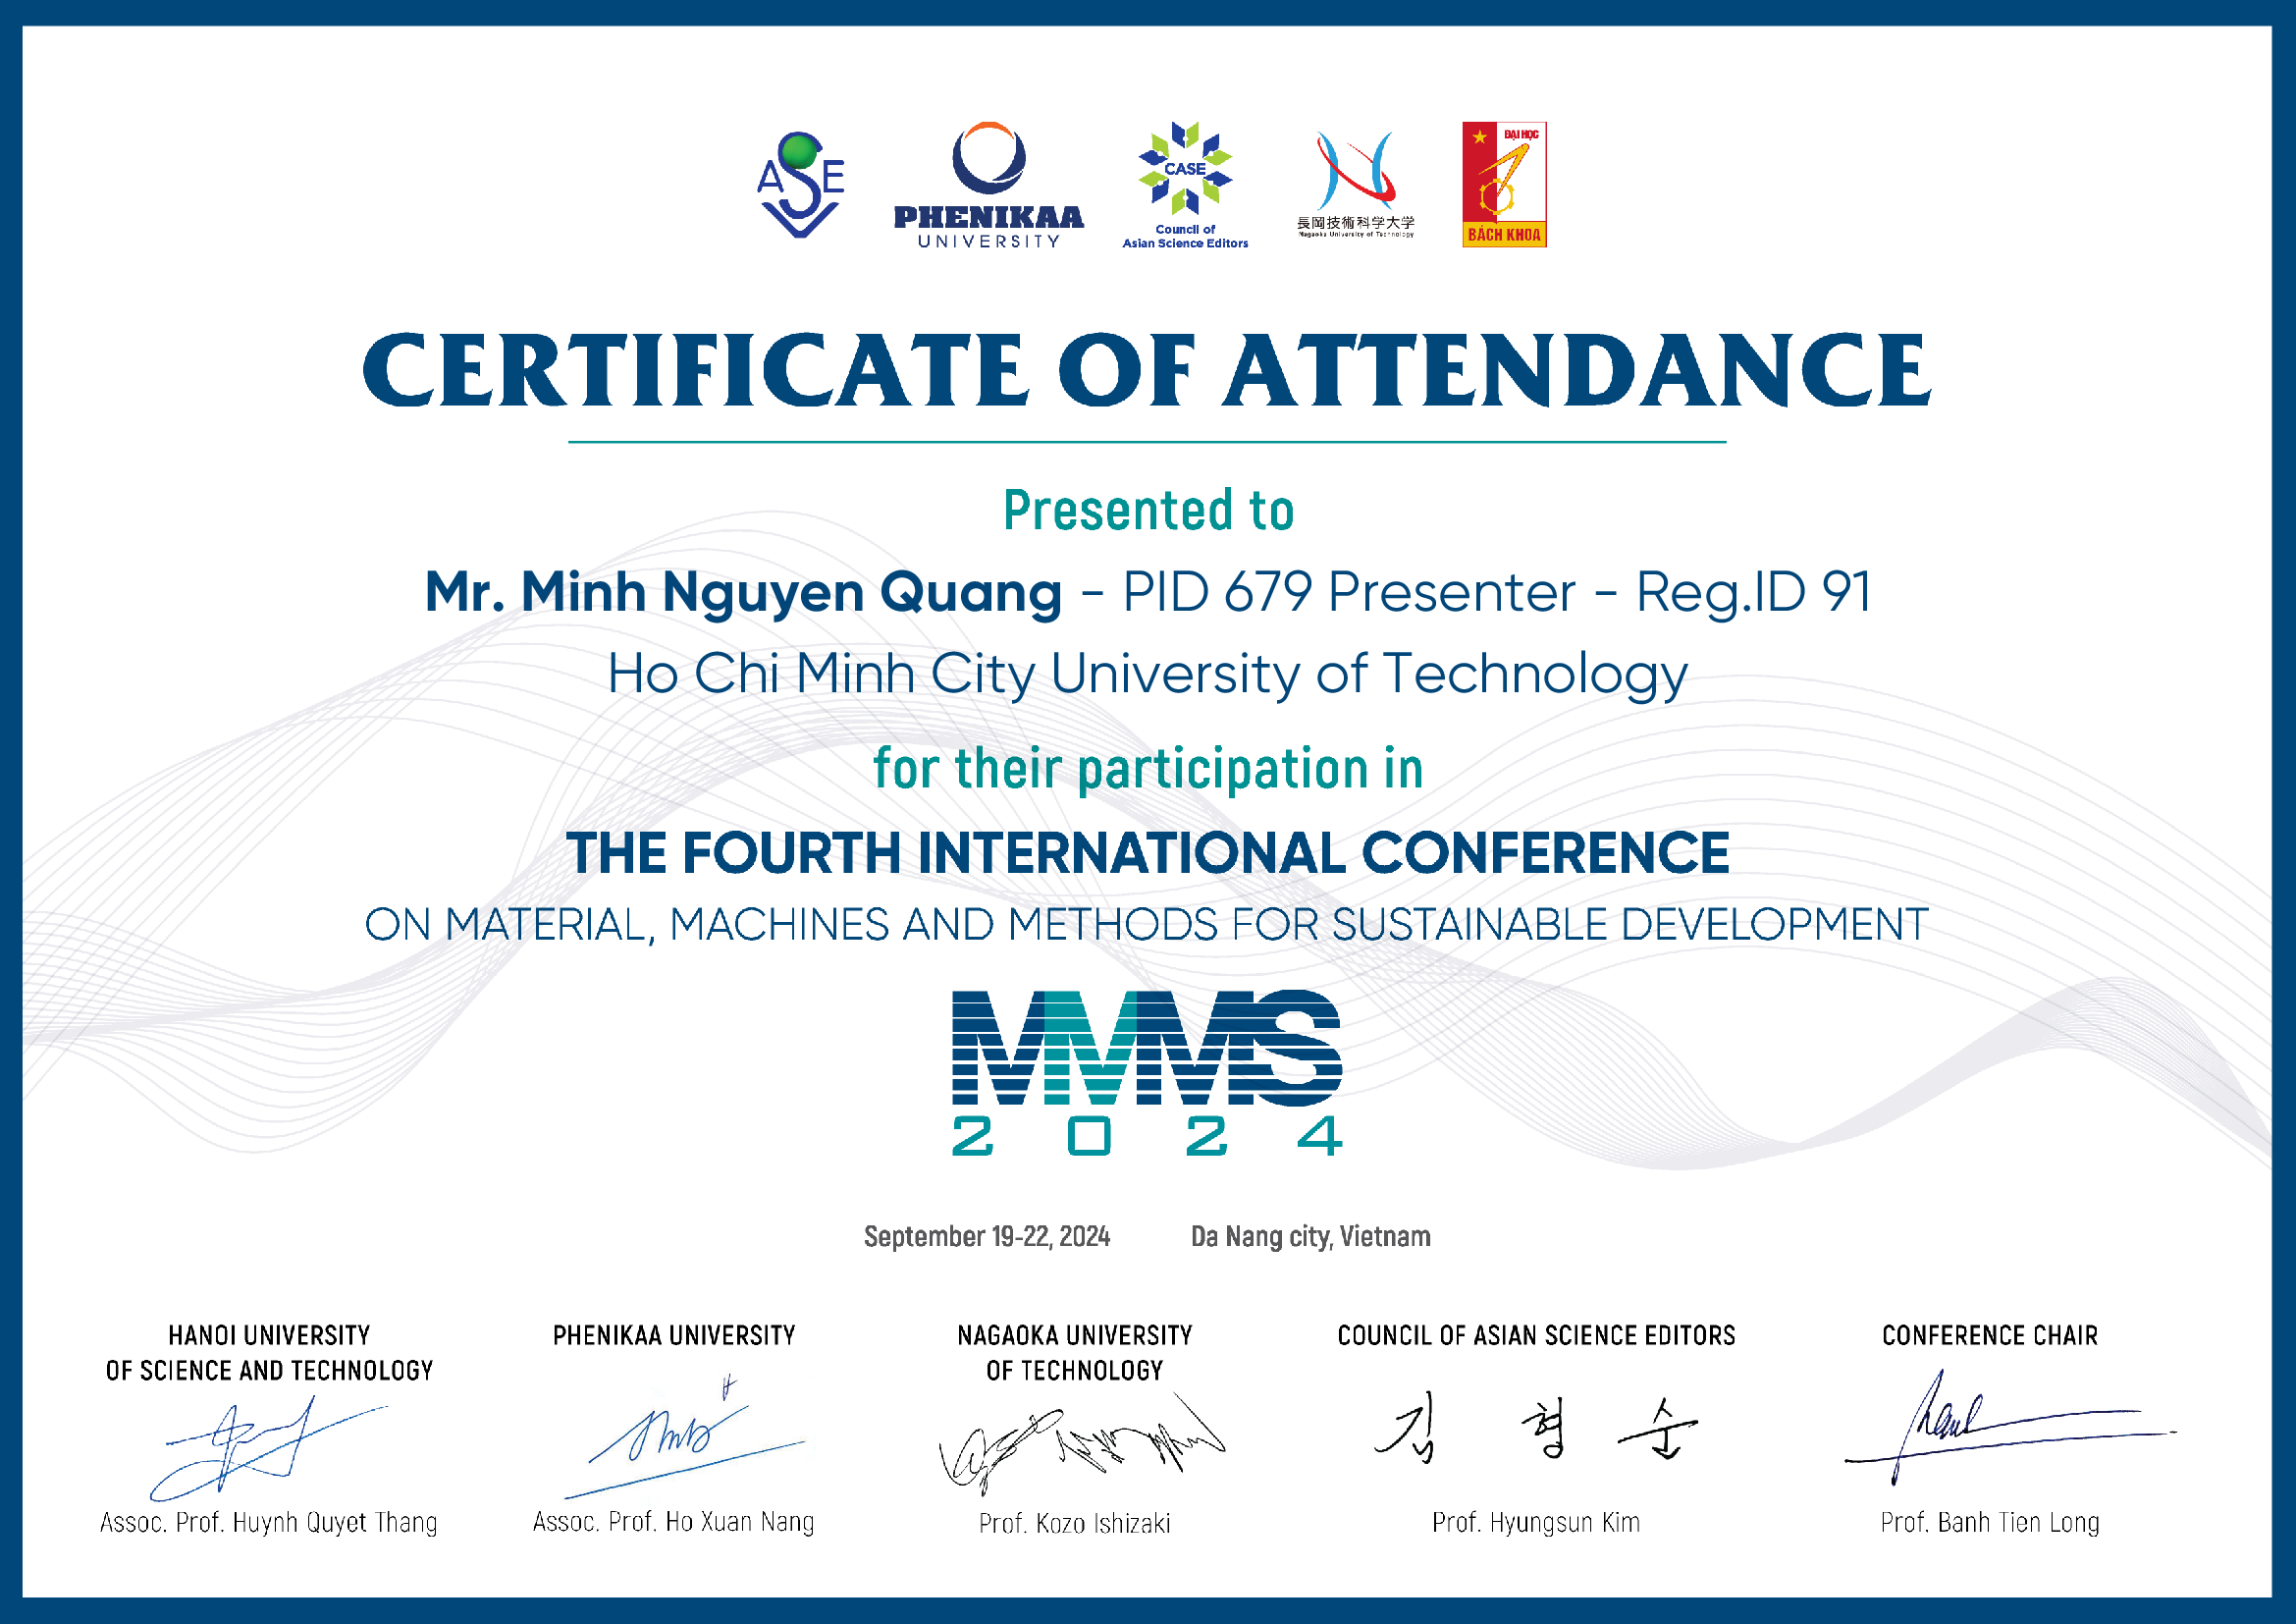
\includegraphics[width=0.8\linewidth, height=0.3\textheight]{images/present.png}
            \vspace{0.6cm}
            \caption{Chứng nhận đã thuyết trình ở hội nghị MMMS2024 của đề tà}
        \end{figure}
    
        \begin{figure}[H]
            \centering
            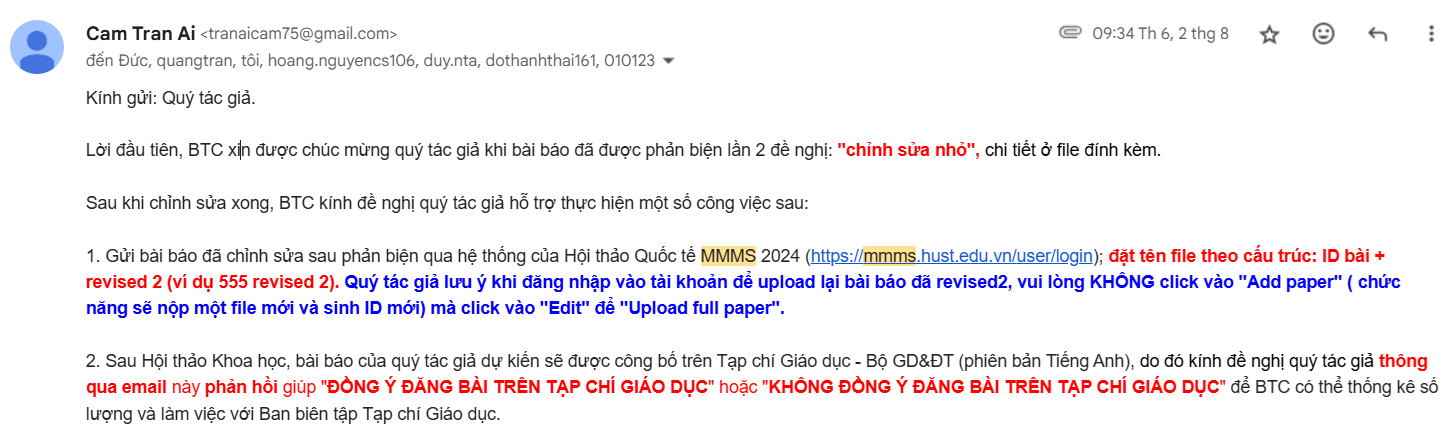
\includegraphics[width=0.8\linewidth]{images/email.png}
            \vspace{0.6cm}
            \caption{Chứng nhận đã thuyết trình ở hội nghị MMMS2024 của đề tà}
        \end{figure}
    \subsection{Thảo luận}
        Tuy nhiên, hệ thống cũng còn tồn đọng nhiều khiếm khuyết, với những khuyết điểm tới từ hiệu suất và tính hoàn thiện của hệ thống cần được khắc phục trong tương lai
        \begin{itemize}
            \item \textit{Chưa có những đánh giá chuyên sâu:} Đánh giá chuyên sâu về hiệu suất và hiệu quả của hệ thống là cần thiết để đảm bảo rằng nó đáp ứng được các yêu cầu và mục tiêu đề ra. Cần tiến hành các đánh giá kỹ thuật và trải nghiệm từ người dùng để cải thiện và điều chỉnh hệ thống.
            \item \textit{Chưa có phân tích chi tiết về dữ liệu:} Dữ liệu thu thập được cần được phân tích chi tiết để đưa ra những kết luận và hướng đi cụ thể. Điều này giúp cải thiện hiệu suất và hiệu quả của hệ thống, từ đó tối ưu hóa trải nghiệm người dùng.
            \item \textit{Chưa có sự cập nhật kịp thời:} Một số nguồn dữ liệu đã từ năm 2021,2022 chưa có sự cập nhật kịp thời theo xu hướng phát triển ngày càng nhanh chóng của xã hội. Cần có sự cập nhật kịp thời về dữ liệu và thông tin để đảm bảo rằng hệ thống luôn cung cấp thông tin chính xác và đáng tin cậy cho người dùng. Điều này giúp tăng tính hấp dẫn và giữ chân người dùng.
            \item \textit{Chưa thật sự tối ưu hóa cho học sinh Việt Nam} Hệ thống chưa thực sự tối ưu hóa cho học sinh Việt Nam, đặc biệt trong việc cải thiện trọng số mô hình để thật sự tương thích với  người dùng Việt Nam. Cần tiến hành nghiên cứu và điều chỉnh để tối ưu hóa hệ thống.
        \end{itemize}